%!TEX root = Main.tex
\documentclass[Main]{subfiles}

\begin{document}

\section{Design, implementation and test setup} % (fold)
\label{sec:design_implementation_test_setup}

	\subsection{System Description}
		The main functional blocks of the system are shown in Figure \ref{fig:sysDesc}. 
		CO$_2$ emission data is acquired from the FTP server by the CO$_2$ Emission Indicator (CEI) application. 
		The CEI application determines whether the emission is high or low and transmits the corresponding control message to the ZigBee LED device. 
		The Sequence Executor Tool (SET) is used by the CEI application for managing the communication with the ZigBee LED device. 
		By specifying the address of the SmartAMM server, ZigBee gateway ID and ZigBee LED device ID, the CEI application is able to communicate with the ZigBee LED device.  

		\begin{figure}[H]
		\centering
		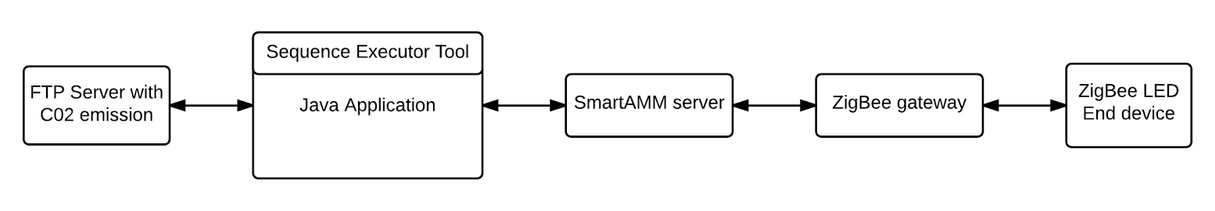
\includegraphics[width=\linewidth]{SystemDescription}
		\caption{System description}
		\label{fig:sysDesc}
		\end{figure}




	\subfile{LevelEstimation} 


	\newpage
	\subsection{Sequence Executor Tool}
		The SET, which is provided by Develco Products, is a Java application able to communicate with ZigBee devices through a SmartAMM server.
		It requires two input files: A \emph{setting} file and a \emph{sequence} file.

		\subsubsection{Setting file}
			The \emph{settings} file is a XML file that contains various settings used in the tool. 
			The most relevant is settings regarding which server the tool should connect to. 
			In this project, the server was hosted on a local PC and the gateway was a USB dongle, which resulted in the following settings:
			\begin{itemize}
				\item gatewayType: ActiveMQ
				\item portNo: 62000
				\item hostName: localhost
			\end{itemize}

		\subsubsection{Sequence files}
			The \emph{sequence} file is also an XML file, specifying the sequence of telegrams to be sent to the ZigBee device, including gateway and device IDs. 
			It also specifies how to determine whether the telegram was successfully receive. 
			In this project positive acknowledgment are used as an indicator for successful transmission.
			In \ref{sec:appendix_a} the XML files for authorizing the LED device on the network, and setting the LED green is shown.
			Each sequence file contains the following items: 
			\begin{itemize}
				\item General sequence descriptions
				\item Substitute texts
				\item Steps
			\end{itemize}
			The general description contains information like sequence name, author, tool version etc.
			The substitute texts are a smart feature in the tool. 
			These allows the user to easily change certain fields in the steps. 
			A great example of this is the sequence file specifying setting the LED red or green.
			Instead of editing directly in the telegram defined in the step section, only the substitute texts need to be changed in order to set the LED red or green. 

			The last items in the sequence files are steps. 
			In both files shown in Appendix A there are two steps. 
			The first step in both files is used to connect to the gateway.
			The second step is used to transmit either an authorization telegram or a LED setting telegram.
			Each step contains a textual representation of the telegram to be transmitted, receive filters, an approval section and a general step description including a timeout interval.

			The receive filter is used to sort incoming telegrams, so that the correct telegram is used to verify the transmission status. 
			In the authorizing sequence, the receive filters sort for a device announce from the LED device with the correct ID.
			
			The approval fields are used to validate the status of the telegram that gets through the receive filters. 
			In the Set LED Green sequence the received telegram must contain a \emph{Status} field with the value \emph{Success}.

			Given the sequence files, the tool is able to differentiate between \emph{Success}, \emph{Failure} and \emph{Timeout}.
			If no telegram passes through the receive filters within the timeout interval, the end status will be \emph{Timeout}.
			If a telegram passes through the receive filters but does not fulfill the approval fields, the end status will be \emph{Failure}.
			And if everything goes well, the end status is \emph{Success}.

		\subsubsection{Application interface}
			The SET is available as a .jar file, and can thus be included in a Java application, from which the main method of the SET can be called.


	\subsection{CO$_2$ Emission Indicator Application}
		The CEI application developed in this project is a Java based command line application. 
		Using Java, eases the use of the SET, since this is also Java based. 
		Additionally, Java is a platform independent language, meaning that the application can be run on all platforms. 
		In the following subsections the main implementation concepts is presented.

		\subsubsection{Application Flow}
		\label{sub:application_flow}
			The application flow is split into two parts. 
			In code snippet \ref{code:program_flow} a pseudo code for the program flow is shown.
			Initially and only once the application will authorize the LED device on the network.
			Afterwards the application will download data from the FTP server, parse the data and set the LED red or green based on the parsed data.
			This is done approximately every 5 minutes, since new data is available from the FTP server.

			\begin{figure}[H]
				\begin{lstlisting}[caption=Program Flow, style=Code-C, label=code:program_flow]
					// Authorize ZigBee LED device
					run SequenceExecutorTool with Authoritation sequence

					// Update LED
					while() {
						CO2Level = GetCO2EmissionData from FTP server
						if (CO2Level > highThreshold)
							run SequenceExecutorTool with Red blinking sequence
						else if (CO2Level < lowThreshold)
							run SequenceExecutorTool with Green blinking sequence
						else
							//Do nothing - hysteresis
						Sleep for 4 minutes
					}
				\end{lstlisting}
			\end{figure}
				

		\subsubsection{Data Collection}
		\label{sub:data_collection}
			To download the data from the FTP server a FTPClient\cite{FTPClient:Online} is used. 
			In code snippet \ref{code:download_co2_data} the pseudo code for getting data from the FTP server is shown. 
			An connection is established with the FTP server, and the necessary login is provided.
			Once the login is accepted, the file containing the CO$_2$ data of the day is downloaded and parsed, and the FTP connection is disconnected.

			\begin{figure}[H]
				\begin{lstlisting}[caption=Download CO2 data, style=Code-C, label=code:download_co2_data]
					server = "ftp.energinet.dk";
	        		port = 21;
					FTPClient.connect(server,port);
					FTPClient.login(username,password);

					date = getTime formatted as "yyyyMMdd";
					remoteFile = "/Onlinedata/"+date+"_onlinedata.txt"

					inputStream = FTPClient.retrieveFileStream(remoteFile);

					mostRecentCo2Data = parseFTPFile(inputStream);

					FTPClient.completePendingCommand();
					FTPClient.logout();
					FTPClient.disconnect();
				\end{lstlisting}
			\end{figure}


			\paragraph{Data Parsing} % (fold)
			\label{par:data_parsing}
				The data retrieved from the FTP server is a file containing data for the day. 
				It is organized as a table with 20 columns, with a row for every data entry, which is every 5 minutes.
				In order to retrieve the most recent data the very last row of the table is used.
				The CO$_2$ emission data is in column 17.
			% paragraph data_parsing (end)

		\subsubsection{Using the SET} % (fold)
		\label{sub:using_sequence_executor_tool}
			The SET was not develop to be embedded in another application, and thus is not very user friendly in that sense.
			By calling the main method of the SET, the only feedback from the SET is logs written to the console. 
			In order to be able to use these logs as a feedback, the output is redirected to the CEI.
			By using the feedback, it is possible to monitor if the sequence succeeds, fails or times out.

			\paragraph{Timeout and retransmissions} % (fold)
			\label{par:timeout_and_retransmissions}
				Unfortunately the SET seems to time out every time, even though the transmission actually succeeds.
				This means that a smart retransmission scheme cannot be implemented in the CEI. 
				Instead the \emph{maxRetransmissions} field in the sequence files can be set, to enable retransmissions, if wanted. 
				In this project \emph{maxRetransmissions} is set to 2, meaning that when the SET times out, the telegram will be retransmitted maximum 2 times, giving a total of 3 transmitted telegrams.

				This gives an unnecessary transmission overhead if the telegram is received correctly, but this is the necessary cost to increase certainty about that the telegram is received.
			% paragraph timeout_and_retransmissions (end)
		% subsection using_sequence_executor_tool (end)

	\subsection{Communication Protocols}
		The system utilizes several different communication technologies.

		\subsubsection{FTP}
			The File Transfer Protocol is used to fetch CO$_2$ data from the Danish Transmission System Operator server.
			FTP is a standard network protocol used to transfer files between hosts on a TCP-based network\cite{FTPWikipedia:Online}.
			FTP is built on a client/server architecture and uses separate control and data connections between the client and the server\cite{TCPIPProtocol}.
			Authentication is in this project handled by a user name and password.  


		\subsubsection{SmartAMM}
			SmartAMM is a proprietary protocol and server architecture developed by Develco Products A/S. 
			SmartAMM makes it possible to monitor and control electrical appliances and energy consumption via smart meters.
			Is is based on the use of ZigBee, and achieves remote control of ZigBee devices through a gateway\cite{SmartAMM:Online}.

			ZigBee telegrams are wrapped inside of the SmartAMM protocol and transmitted to the gateway, which relays the ZigBee telegram to the ZigBee device as seen in \ref{sec:appendix_a}.


		\subsubsection{ZigBee}
			As the LED device is ZigBee enabled, this is the technology of choice for communication. 
			ZigBee is a low power and low data rate wireless protocol for personal area networks. 
			The lower layers(MAC and PHY) of the protocol are based on the IEEE 802.15.4 standard\cite{ZigBeeSpec}, whereas higher layers such as network and application have been defined by the ZigBee Alliance.
			ZigBee features a range of different application profiles including Home Automation (HA), Building Automation, Light Link, Smart Energy etc\cite{ZigBeeApplicationProfiles:Online}.
			The LED device and gateway are both setup as HA devices. 

			\paragraph{Commissioning} % (fold)
				Commissioning is the term used for establishing a ZigBee network.
				A ZigBee network must contain one ZigBee Coordinator (ZC) and one or more ZigBee Routers(ZR) and ZigBee End Devices(ZED). 
				The ZC is responsible for maintaining the network by transmitting beacons, which provide information to other nodes (both associated and non-associated) about the network.

				One of the non-sleeping devices in a ZigBee network must act as the trust center, which is usually handled by the ZC. 
				It is the responsibility of the trust center to authorize new device that wish to join the network.

				In this project the ZigBee network is very simple as is consists only of two nodes, the gateway and the LED. 
				The gateway is the ZC and acts as trust center as well, whilst the LED is a ZED.
				The LED device is authorized to join the network by adding it's MAC address to the trusted table of the trust center. 
				This is performed by the CEI application.
				When the LED device attempts to join the network, the address is recognized as trusted and the device is able to join the network. 

				A consequence of such a simple approach is that the CEI application must be aware of the MAC address of the LED device beforehand. 
				The address must either be known at compile time, or be input by the user, which would require a user interface. 
				However in order to implement a proof-of-concept system, this simple approach is appropriate. 			
			\label{par:commissioning}
			
			% paragraph commissioning (end){Commissioning}



			\paragraph{Security} % (fold)
				In a ZigBee network the security is mandated by the application profile in use, in this case this is the HA profile.
				A trust center link key has been defined in the HA profile\cite{HASpec}:
				\begin{equation}
					0x5A\ 0x69\ 0x67\ 0x42\ 0x65\ 0x65\ 0x41\ 0x6C\ 0x6C\ 0x69\ 0x61\ 0x6E\ 0x63\ 0x65\ 0x30\ 0x39	
				\end{equation}
				
				The trust center must pick a network key. The network key is sent to new devices encrypted with the trust center link key.
				A 128-bit AES encryption is used.
				This is the lowest security setting in the HA profile, and has been chosen for this project. 
				Alternatively pre-configured link keys can be specifically associated with the different devices of a network.
			\label{par:security}
			
			% paragraph security (end)

			
			% subsection subsection_name (end)


		% Web protokoller - Ivan Starter
		% Det sidste



% section design_implementation_test_setup (end)
\end{document}